\section{Methodology}
\begin{figure*}
\vspace{10pt}
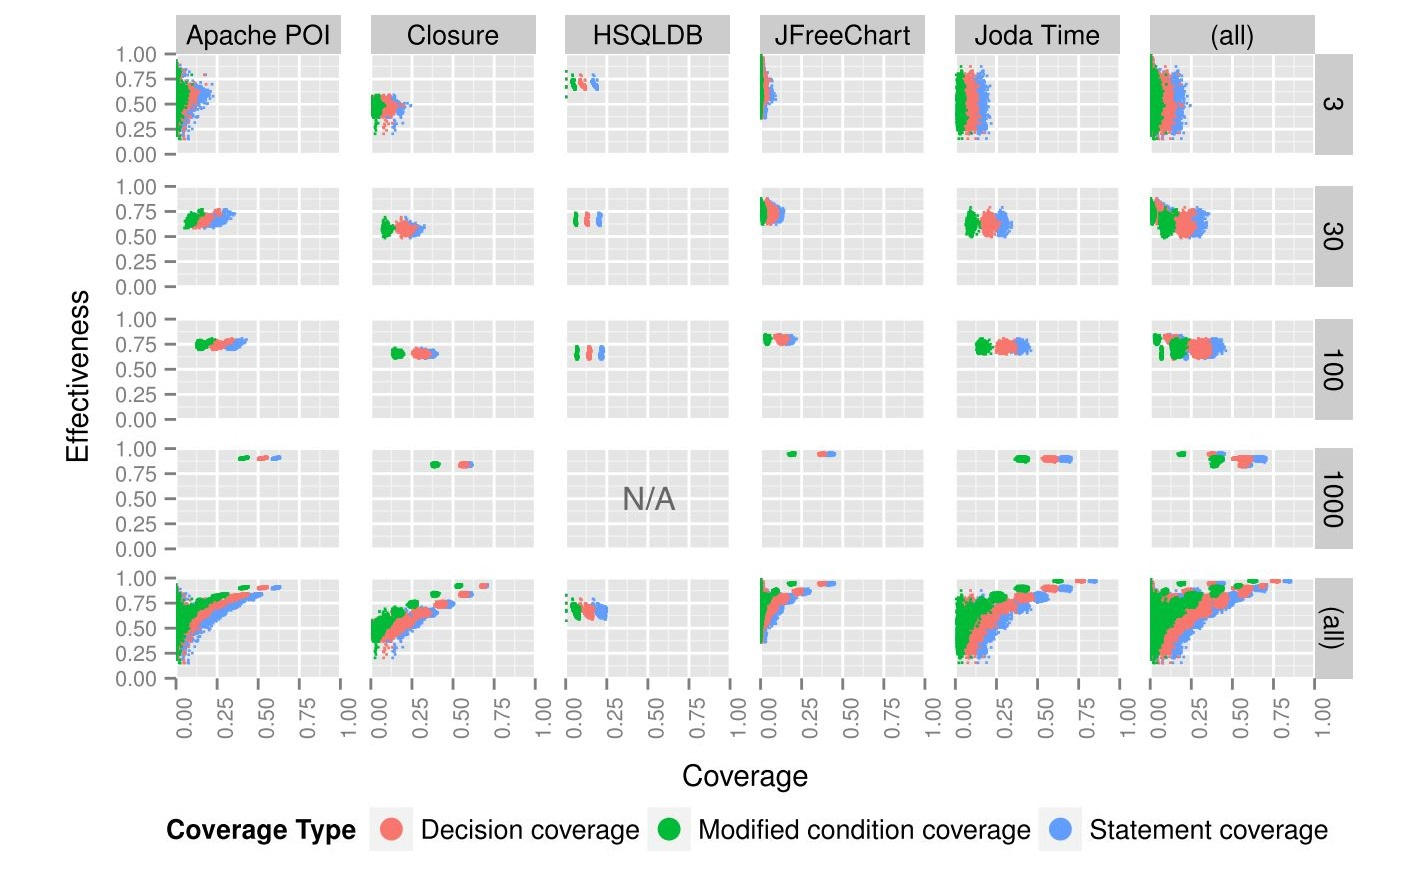
\includegraphics[width=\textwidth,height=7cm]{Figures/Coverage_result.JPG}
\caption{Normalized effectiveness scores (left axis) plotted against coverage (bottom axis) for all subjects. Rows show the results for one suite size; columns show the results for one project.}
\label{f1}
\end{figure*}

\subsection{Terminology}
\begin{itemize}
    \item \textbf{Master suite:} Test suite written by developers of a subject program. The all other suites are strict subsets of this suite.
    \item \textbf{Mutant and Equivalent Mutant: }A mutant is a new version of the program that is created by making a small syntactic change to the original program. If resulting mutant produce the same output, it is called an equivalent mutant.
    %(i.e. negating a branch condition, or removing a method call etc.).
\end{itemize}

\subsection{Subject Program}
They have used a number of criteria to select these projects. 
\begin{itemize}
    \item Large projects on Java (on the order of 100,000 SLOC), actively developed.%novelty and generalizability
    \item Large number of test methods (on the order of 1,000). %generate reasonably sized random test suites
    \item Ant as a build system and JUnit as a test harness, to automate data collection.
\end{itemize}

\subsection{Generate Faulty Program}
Inozemtseva et al. \cite{inozemtseva2014coverage} used the open source tool \textbf{PIT} \cite{coles2016pit} to generate large number of mutants and run the program’s test suite on each one. If the test suite fails when it is run on a given mutant, the suite is said to kill that mutant, else it is equivalent. A test suite’s mutant coverage is the fraction of mutants that it kills.

\subsection{Generate Test Suite}
%reflection API
For each program, they have identified all of the test methods in the master suite. Then generated new test suites of fixed size by randomly selecting a subset of these methods without replacement. They made 1,000 suites for the following sizes: 3 methods, 10 methods, 30 methods, 100 methods, and so on. This resulted in a total of 31,000 test suites.

\subsection{Measuring Coverage}
Inozemtseva et al. used the open source tool \textbf{CodeCover} \cite{scheller2008codecover} to measure coverage. They used two effectiveness measurements in this study: normalized and non-normalized. The normalized effectiveness measurement is the number of mutants a test suite detected divided by the number of non-equivalent mutants it covers. For non-normalized results, see \cite{inozemtseva2014coverage}
